\documentclass[12pt,a4paper]{article}

\usepackage[T1,T2A]{fontenc}
\usepackage[utf8]{inputenc}
\usepackage[english, russian]{babel}
\usepackage{indentfirst}
\usepackage{misccorr}
\usepackage{graphicx}
\usepackage{amsmath}
\usepackage{graphicx}
\usepackage{float}
\usepackage[left=20mm,right=10mm, top=20mm,bottom=20mm,bindingoffset=0mm]{geometry}

\setlength{\parskip}{6pt}
\DeclareGraphicsExtensions{.png}

\begin{document}

    \begin{titlepage}
        \begin{center}
            \large
            Санкт-Петербургский политехнический университет\\Петра Великого\\
            \vspace{0.5cm}
            Институт прикладной математики и механики\\
            \vspace{0.25cm}
            Кафедра «Прикладная математика»
            \vfill
            \textsc{\LARGE\textbf{Отчет по лабораторной работе №8}}\\[5mm]
            \Large
            по дисциплине\\"Математическая статистика"
        \end{center}
        \vfill
        \begin{tabular}{l p{175} l}
            Выполнила студентка\\группы 3630102/80201 && Деркаченко Анна Олеговна
            \vspace{0.25cm}
            \\Проверил\\доцент, к.ф.-м.н. && Баженов Александр Николаевич
        \end{tabular}
        \vfill
        \begin{center}
            Санкт-Петербург\\2021 г.
        \end{center}
    \end{titlepage}

\newpage
\begin{center}
    \tableofcontents
    \setcounter{page}{2}
\end{center}
\newpage
\begin{center}
    \listoffigures
\end{center}

\newpage
\section{Постановка задачи}
Необходимо:
\begin{enumerate}
    \item Провести дисперсионный анализ с применением критерия Фишера по данным регистраторов для одного сигнала
    \item Определить области однородности сигнала, переходные области, шум/фон
    \item Взять длину сигнала равной 1024
\end{enumerate}

\section{Теория}
\subsection{Величины дисперсионного анализа}
Необходимо вычислить следующие величины:
\begin{enumerate}
    \item \textit{Внутригрупповая дисперсия}
        \begin{equation}
            s_{IntraGroup}^2=\frac{1}{k}\sum_{i=1}^ks_i^2=\frac{1}{k}\sum_{i=1}^k\frac{\sum_{j=1}^n(x_{ij}-X_{cp})^2}{k-1},
        \end{equation}
        где $X_{cp}$ - среднее для части выборки, $k$ - количество частей выборки, $n$ - количество элементов в рассматриваемой части выборки.\\Внутригрупповая дисперсия является дисперсией совокупности и рассматривается как среднее значение выборочных дисперсий.
    \item \textit{Межгрупповая дисперсия}
        \begin{equation}
            s_{InterGroup}^2=k\frac{\sum_{i=1}^k(X_{i_{cp}}-X_{cp})^2}{k-1},
        \end{equation}
        где $X_{1_{cp}},X_{2_{cp}},...,X_{k_{cp}}$ - среднее значение для подвыборок, $X_{cp}$ - среднее значение этих cредних значений подвыборок
    \item \textit{Значение критерия Фишера}
        \begin{equation}
            F=\frac{s_{InterGroup}^2}{s_{IntraGroup}^2}
        \end{equation}
\end{enumerate}

\subsection{Ход работы}
\begin{enumerate}
    \item Извлечь сигнал из исходных данный в файле wave\_ampl.txt. Так как сигнал имеет длину 1024, выбрать начальный индекс, кратный длине сигнала
    \item Построить гистограмму с столбцами:
        \begin{itemize}
            \item фон - столбец с наибольшим значением
            \item сигнал - второй по величине столбец после фона
            \item переходы - столбцы с малыми значениями
        \end{itemize}
    \item Устранить явные выбросы, то есть сгладить сигнал, используя медианный фильтр с переназначением выброса как среднего арифметического его соседеней
    \item Разделить сигнал на области: сигнал, фон, переходные процессы
    \item Определить тип области по критерию Фишера:
        \begin{itemize}
            \item если значение критерия Фишера велико, то эта область переходных процессов
            \item если значение критерия Фишера находится вблизи 1, то эти области однородны
        \end{itemize}
\end{enumerate}

\section{Реализация}
Реализация лабораторной работы проводилась на языке Python в среде разработки PyCharm c использованием дополнительных библиотек:
\begin{itemize}
    \item numpy
    \item matplotlib
    \item math
\end{itemize}

Исходный код лабораторной работы размещен в GitHub-репозитории.

URL: https://github.com/derkanw/Mathstat/tree/main/lab8

\section {Результаты}
Рассматривается сигнал с 2 номером.
\begin{figure}[H]
    \centering
    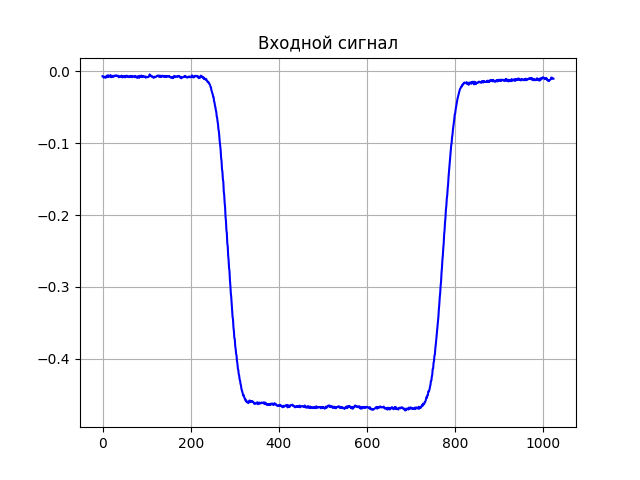
\includegraphics[scale=0.8]{signal.png}
    \caption{График входного сигнала}
\end{figure}
\begin{figure}[H]
    \centering
    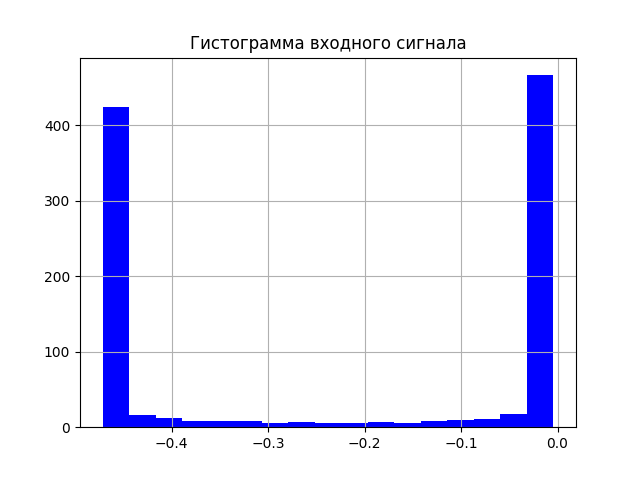
\includegraphics[scale=0.8]{hist.png}
    \caption{Гистограмма входного сигнала}
\end{figure}
\begin{figure}[H]
    \centering
    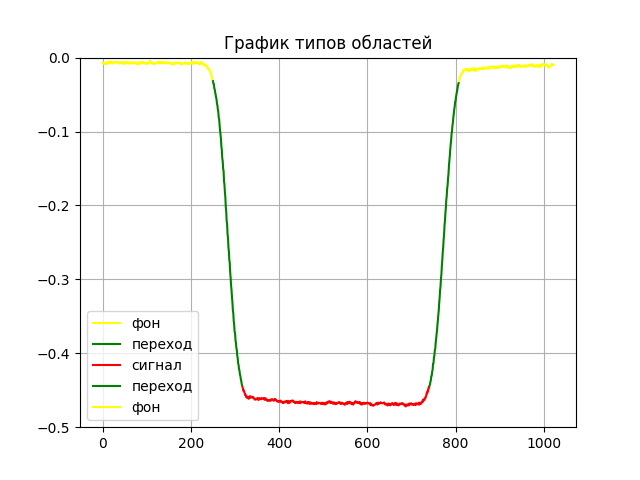
\includegraphics[scale=0.8]{zones.png}
    \caption{График разделения сигнала на однородные области}
\end{figure}
\begin{table}[H]
    \centering
    \begin{tabular}{|c|c|c|c|}
        \hline
        Область & Тип & Количество разбиений & Критерий Фишера\\\hline
        [0, 250] & Фон & 5 & 0.153571\\\hline
        [250, 317] & Переход & 4 & 17.179199\\\hline
        [317, 741] & Сигнал & 4 & 0.076965\\\hline
        [741, 808] & Переход & 4 & 17.198535\\\hline
        [808, 1023] & Фон & 5 & 1.091278\\\hline
    \end{tabular}
    \caption{Характеристика выделенных областей}
\end{table}

\section{Обсуждение}
Входные данные были разделены на 5 частей: фон, переход, сигнал, переход, фон. При этом по критерию Фишера обе области фона имеют значения, близкие к единице, особенно левая из них, то есть можно заключить, что области достаточно однородны. Области, в которых наблюдается переход, имеют почти равные, но достаточно большие значения критерия Фишера, что говорит о неоднородности областей.

Стоит сказать, что график данных о сигнале почти симметричен относительно вертикали в точке, равной середине длины волны. А также заметно, что сигнал является центральной областью на графике данных. К тому же, при построении графиков не наблюдалось особых выбросов.
\end{document}
